%%%%%%%%%%%%%%%%%%%%%%%%%%%%%
% Supplementary Information %
%%%%%%%%%%%%%%%%%%%%%%%%%%%%%
\captionsetup*{format=largeformat}
\section{JF549 dye photobleaching kinetics}
\label{note:dye_bleaching} 

In our approach to estimating RecB binding times to DNA, the photostability of the fluorescent dye was of primary concern. Since we detect single molecules of RecB bound to DNA, two main photophysical behaviours were liable to cause artefacts in our data:
\begin{enumerate}
    \item Photobleaching (an irreversible loss of fluorescence) would limit the maximum number of frames we can track a DNA-bound RecB for, and would artefactually reduce the fitted binding times since some fluorescent spots might disappear due to photobleaching rather than unbinding from DNA
    \item Blinking (a transient loss of fluorescence) could cause repeated disappearance and reappearance of single molecules, and hence bias the computed binding times
\end{enumerate}

To address these concerns, we computed ensemble-level photobleaching curves by integrating the total fluorescence signal from the cells (Supp. Fig. \ref{SIFig:dye_bleaching}A). After 50 frames of laser exposure, a significant amount of photobleaching was noticeable (27\% $\pm$ 9 of the initial fluorescence remaining). The exact photobleaching rate of the dye in our experimental conditions can be estimated by fitting the photobleaching curve with an exponential decay function of the form $y=a.e^{-k.t}+b$ (with a the amplitude of the fit, k the bleaching rate, and b an offset to account for cellular auto-fluorescence). Since the bleaching rate is expected to mostly depend on experimental parameters that vary between but not within datasets (output laser power, HiLo angle), one bleaching rate was computed per dataset (Supp. Fig. \ref{SIFig:dye_bleaching}B). The true RecB dissociation rates were computed by subtracting the corresponding bleaching rates from the fitted spot disappearance rates.

All experimental photobleaching curves were well-fitted by a mono-exponential decay function. If significant blinking of the dye was occurring, we would expect photobleaching curves to follow more complex kinetics.\cite{} We therefore concluded that in our experimental conditions, the JF549 dye was not experiencing blinking, consistent with previous reports of the dye's outstanding photostability.\cite{}

\clearpage

\section{Formation of RecB spots by the freely diffusing RecBCD-Halo-Gam complex}
\label{note:spurious_spots}



\section{Fitting of the RecB spot lifetime histogram in mutant strains}  % Note: might not be necessary
\label{note:mutants_fitting}


\clearpage

\setlength\intextsep{40pt}

%% SUPPLEMENTARY FIGURES

% Strains table
\begin{supptable}[htbp]
    \centering
    \begin{tabular}{lll}
        \toprule
        Name & Description & Reference\\
        \midrule
        MEK2324 & MG1655, \textit{recB1080::halotag HK022::psfiA-GFP} & \\ % Alessia's article
        MEK2622 & MG1655, \textit{recB::halotag $\Delta$recA} & \\ % = AL133_1, is this published? It should also have a previous MEK number
        MEK2623 & MG1655, \textit{recB::halotag recA::syfp2} & this work\\
        MEK2627 & MG1655, \textit{recB1080::halotag $\Delta$recA} & this work \\
         \bottomrule
    \end{tabular}
    \caption{List of bacterial strains used in this study}
    \label{SItab:strains}
\end{supptable}

% Data analysis pipeline
\begin{suppfigure*}[htbp]
\begin{center}
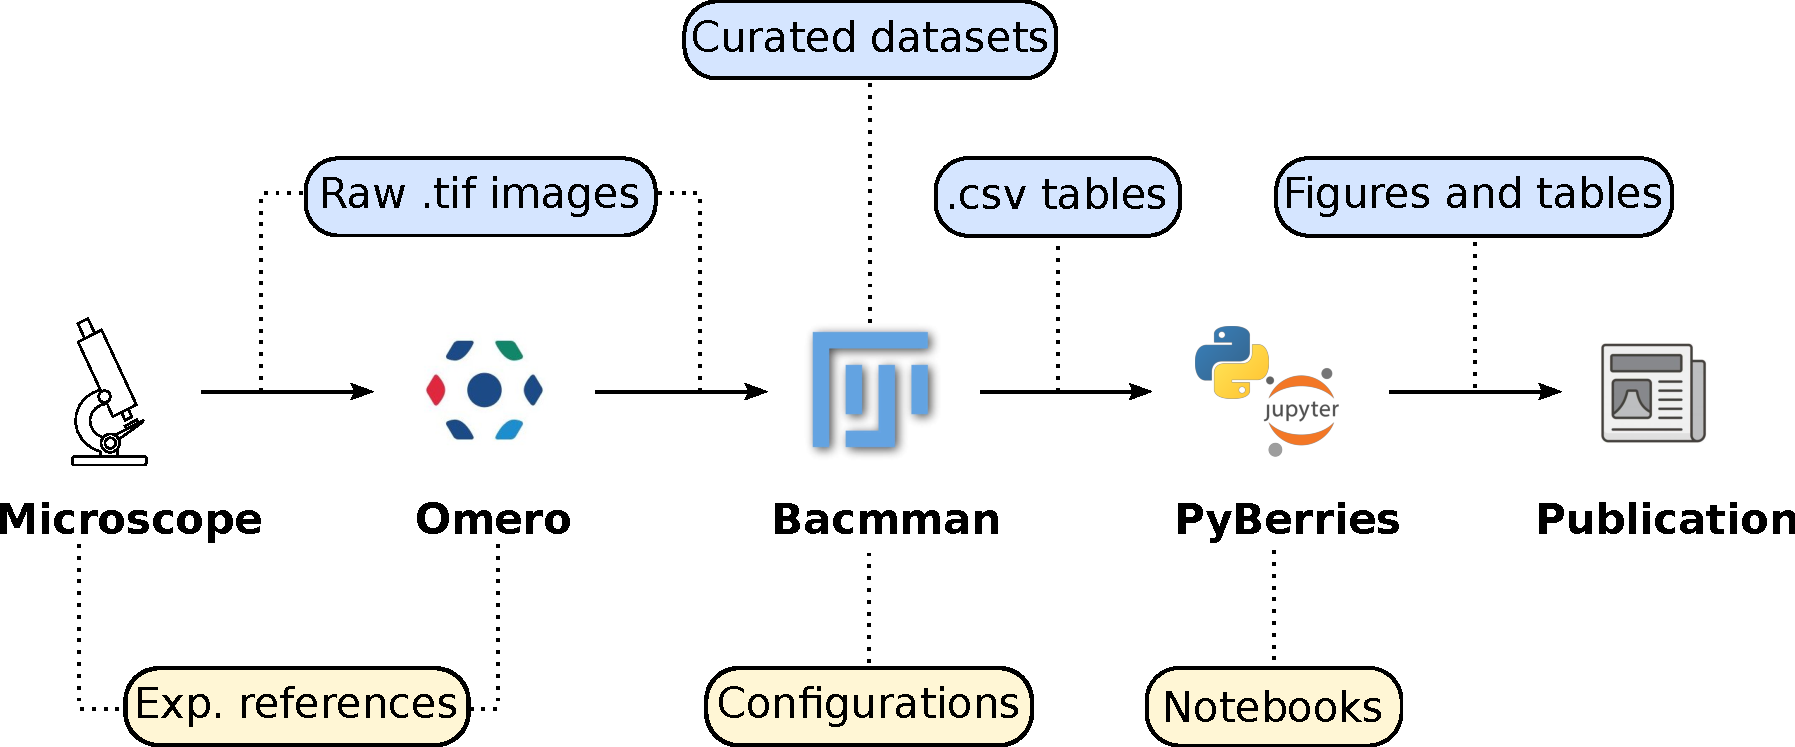
\includegraphics[width=\textwidth]{SI_Figures/Data_analysis_workflow.pdf}
\end{center}
\caption{Data storage and analysis pipeline used in this study. Blue labels indicate stored data and yellow labels indicate code and references that would allow reproducing the different analysis steps.}
\label{SIFig:analysis_workflow}
\end{suppfigure*}

%\clearpage

% Example image of freely diffusing halo-tag + JF549
\begin{suppfigure*}[htbp]
\begin{center}
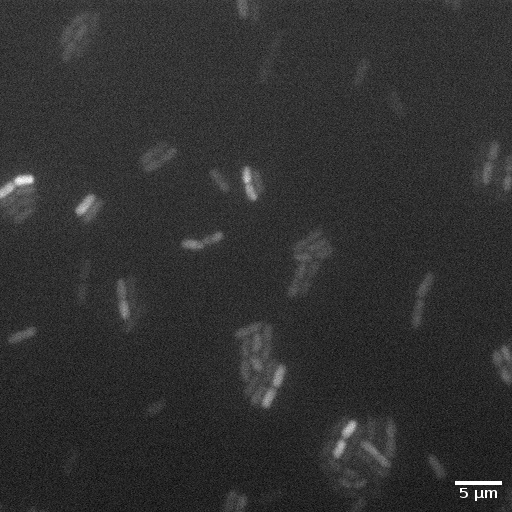
\includegraphics[width=.5\linewidth]{SI_Figures/Free_Halo_image.png}
\end{center}
\caption{Fluorescence image of freely diffusing Halo-tag expressed from a pBAD plasmid in MG1655 \textit{E. coli} cells.}
\label{SIFig:freehalo_image}
\end{suppfigure*}

% Monoexponential fit of WT data, all cipro concentrations
\begin{suppfigure*}[htbp]
\begin{center}
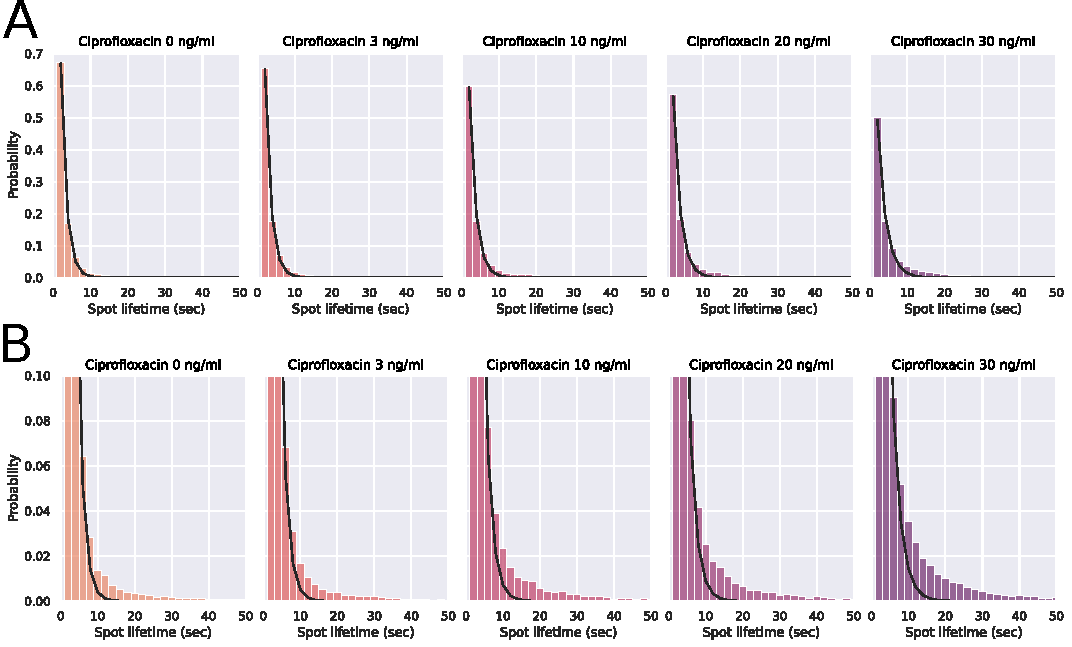
\includegraphics[width=\linewidth]{SI_Figures/Monoexp_fits_cipro.pdf}
\end{center}
\caption{Histograms of RecB spot lifetime (bars) under exposure to ciprofloxacin, with overlaid mono-exponential decay fits ($y=a.e^{-k.t}$, black line).}
\label{SIFig:monoexp_fits}
\end{suppfigure*}

%\clearpage

% Cell length under Gam over-expression, 0 and 30 ng/mL cipro
\begin{suppfigure*}[htbp]
    \begin{center}
    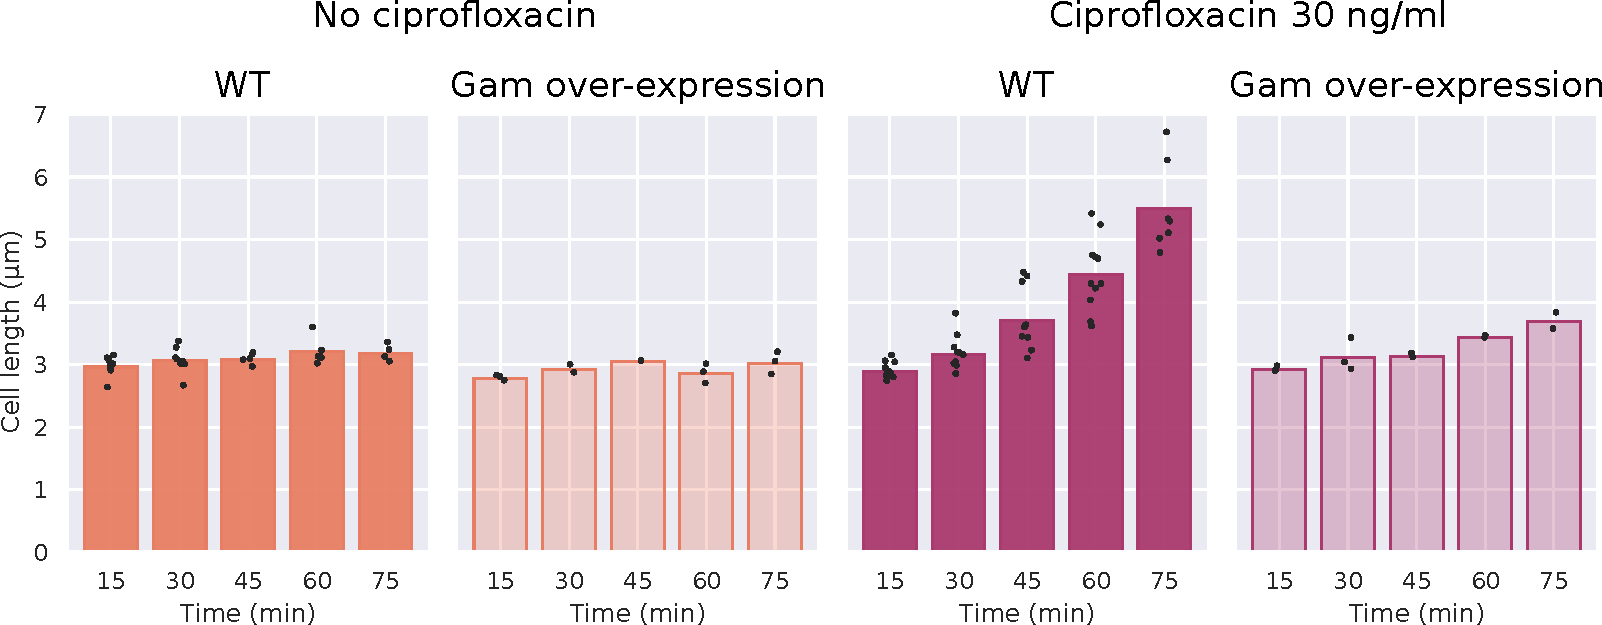
\includegraphics[width=\linewidth]{SI_Figures/Cell_length_Gam.pdf}
    \end{center}
    \caption{Length of cells that over-express Gam or not (WT), under exposure to 0 or 30 ng/mL ciprofloxacin. Black dots show indvidual datasets, and bars the average between them.}
    \label{SIFig:Gam_cell_length}
\end{suppfigure*}

% Photobleaching figure (curves + fitted rates)
\begin{suppfigure*}[htbp]
\begin{center}
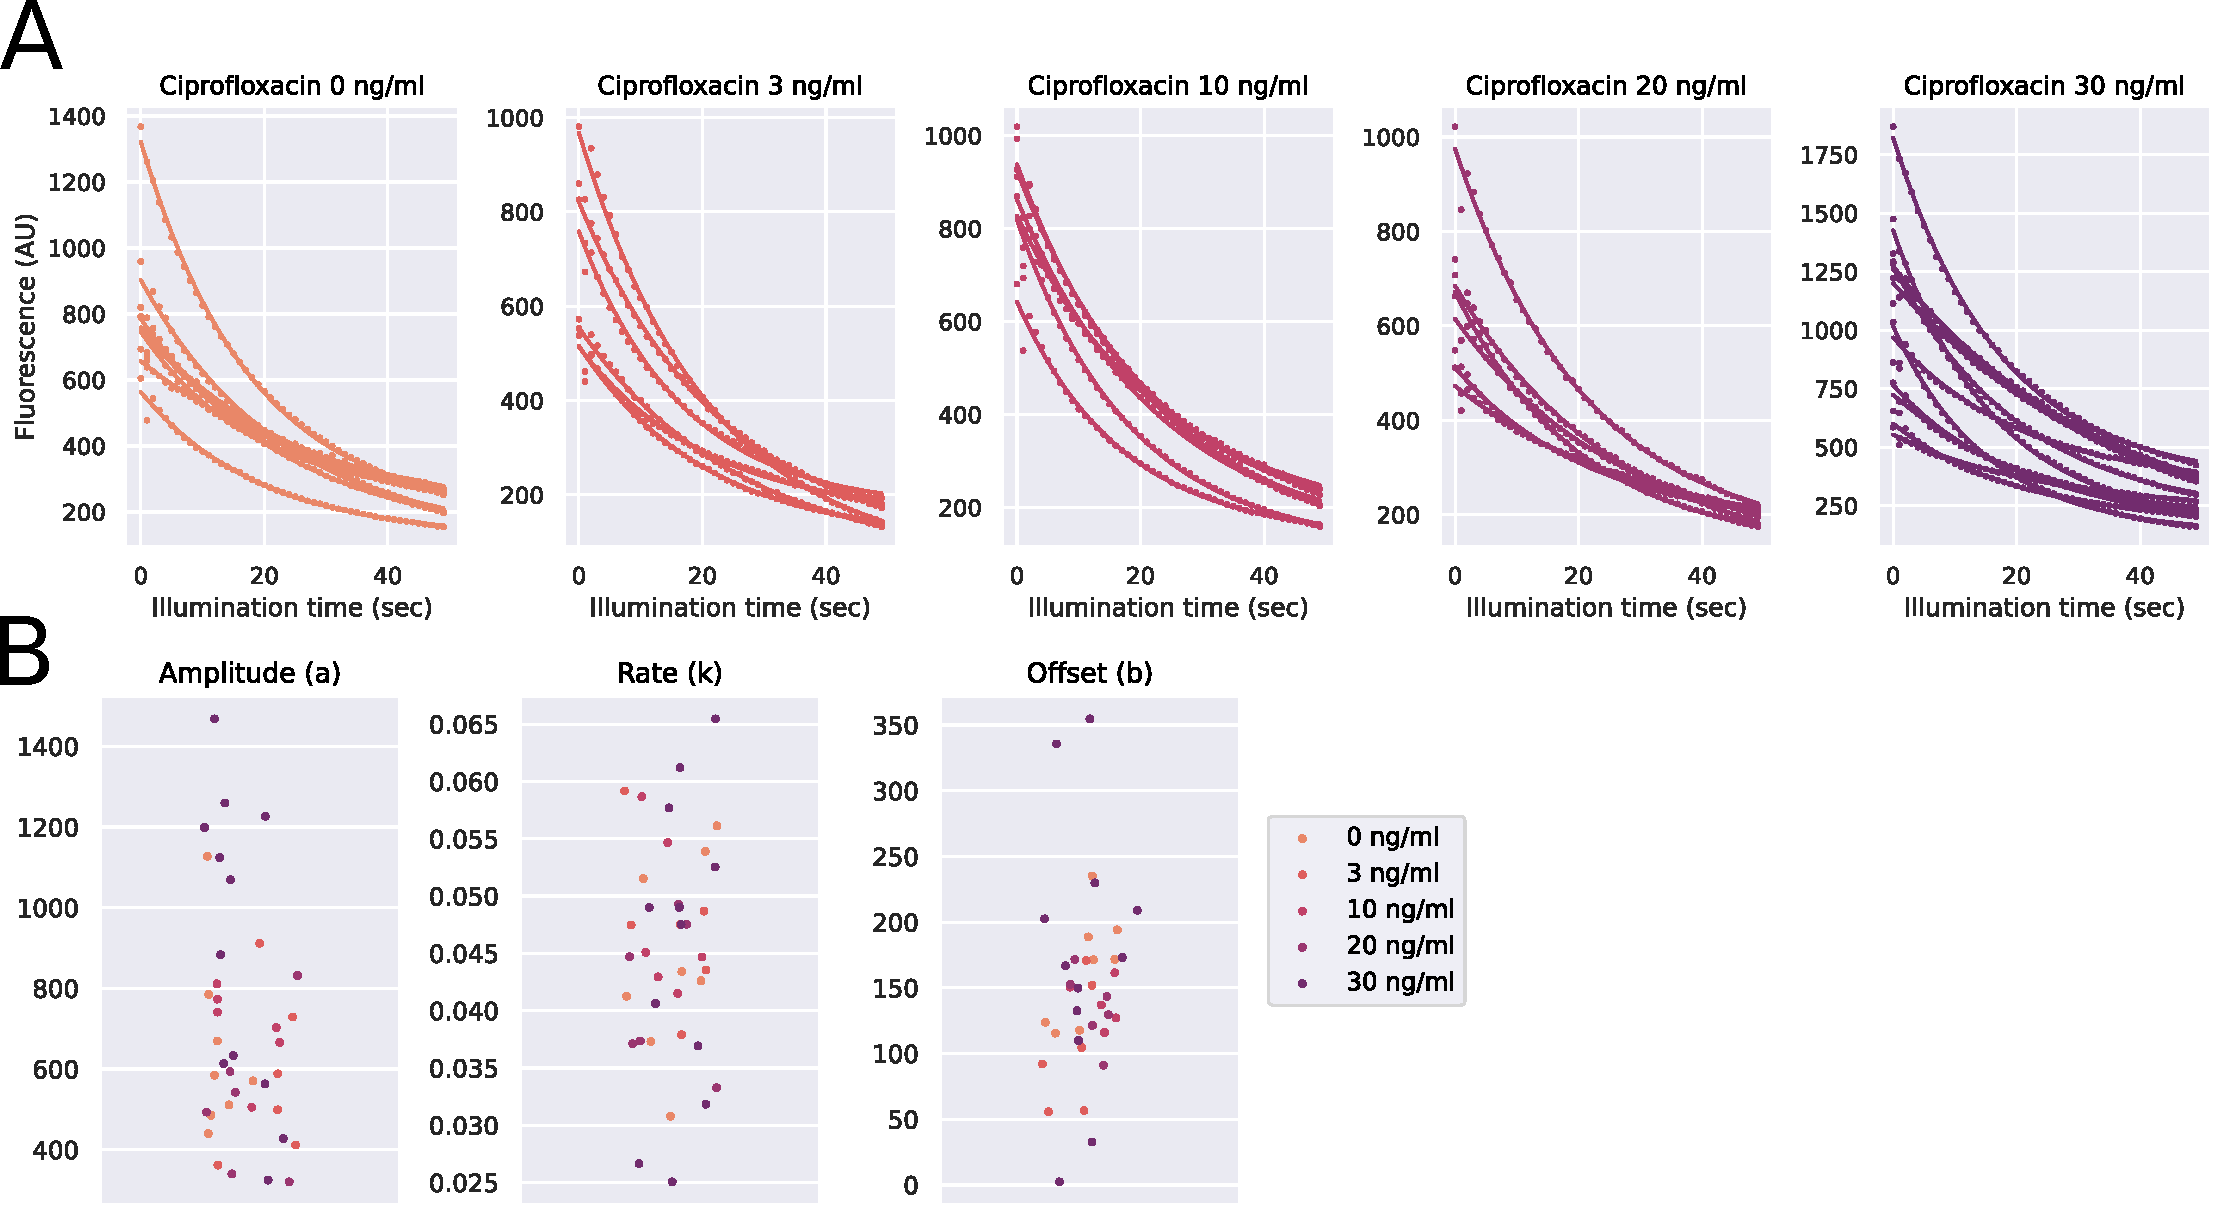
\includegraphics[width=\textwidth]{SI_Figures/SIFig_bleaching.pdf}
\end{center}
\caption{Ensemble-level photobleaching of the JF549 dye. (A) Average background-subtracted fluorescence for 5 independent datasets (solid lines), overlaid with the photobleaching rate fit ($y=a.e^{-k.t}+b$, dotted line). (B) Fitted model parameters for each of the 5 datasets: amplitude (a), offset (b) and photobleaching rate (k).}
\label{SIFig:dye_bleaching}
\end{suppfigure*}


% RecB binding times at different sampling rates
\begin{suppfigure*}[htbp]
\begin{center}
%\includegraphics[width=\textwidth]{}
\end{center}
\caption{}
\label{SIFig:frame_intervals}
\end{suppfigure*}


% Object classification workflow
\begin{suppfigure*}[htbp]
\begin{center}
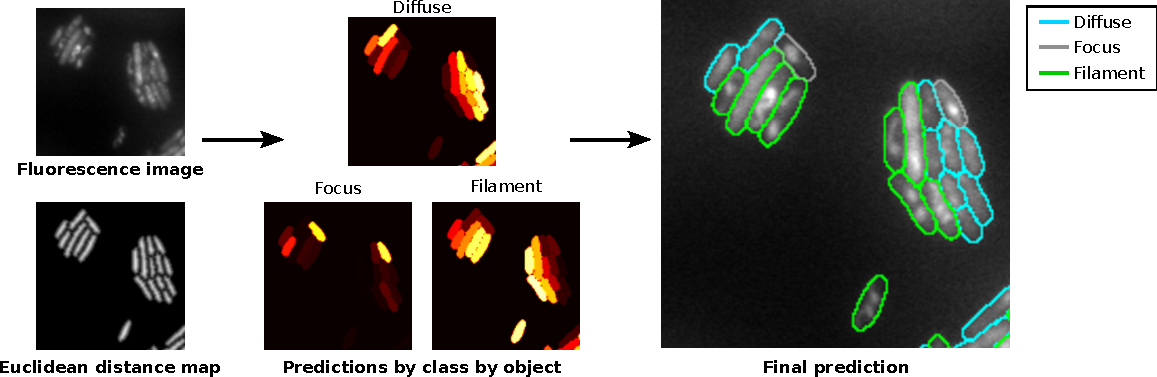
\includegraphics[width=\textwidth]{SI_Figures/ObjectClassifier.pdf}
\end{center}
\caption{Classification of cells according to the RecA structures they contain by our in-house Unet-based deep-learning network.}
\label{SIFig:object_class}
\end{suppfigure*}
